\documentclass[15pt]{article}
\usepackage[utf8]{inputenc}
\usepackage{amsmath}
\usepackage{indentfirst}
\usepackage{graphicx}
\usepackage{subfigure}
\usepackage{float} 
\setlength{\parindent}{2em}
\usepackage{booktabs}
\usepackage{multirow}
\usepackage{geometry}
\usepackage{fancyhdr}
\pagestyle{fancy}
\fancyhf{}
\usepackage{xeCJK}
\usepackage{mathrsfs}
\usepackage{amssymb}
\usepackage{amsfonts,amssymb}

\geometry{a4paper,scale=0.74}
\lhead{Introduction to Algorithm}
\rhead{ENGG 1330}
\begin{document}
Introduction to Algorithm Notes \par
\small{Created by He Entong}
\section{Time Consumption of Bucket Sort}
Since the time consumption of applying INSERTION SORT to every bucket is $O(n_i^2)$, and going through every bucket have time consumption of $\Theta(n)$, we obtain
\begin{equation}
\begin{aligned}
    T(n) &= \Theta(n) + \sum_{i=0}^{n-1} O(n_i^2) \\
    E[T(n)] &= \Theta(n) + \sum_{i=0}^{n-1} O(E[n_i^2]) 
\end{aligned}
\end{equation}

\begin{equation}
\begin{aligned}
    E[n_i^2] &= \sum_{x=0}^{n} x^2 P(n_i = x | \sum_{j=0}^{n-1} n_j = n) \\
    & = \sum_{x=0}^{n} x^2 (\frac{1}{n})^x (\frac{n-1}{n})^{n-x} \\ & = \frac{d^2 t}{dt^2} M_{n_i}(t) \bigg|_{t=0} \\
    M_{n_i}(t) &= \sum_{x=0}^{n} (\frac{1}{n} e^{t})^x (\frac{n-1}{n})^{n-x} \\ 
    & = (\frac{1}{n} e^{t} + \frac{n-1}{n})^n \\
    E[n_i^2] &= \frac{d^2 t}{dt^2} M_{n_i}(t) \bigg|_{t=0} \\
    & = e^t (\frac{1}{n} e^t + \frac{n-1}{n})^{n-1} + \frac{n-1}{n} e^{2t} (\frac{1}{n}e^t + \frac{n-1}{n})^{n-2} \bigg|_{t=0} \\ 
    &= 2- \frac{1}{n}
\end{aligned}
\end{equation}
Substitute (2) into (1) we obtain
\begin{equation}
\begin{aligned}
    E[T(n)] &= \Theta(n) + \sum_{i=0}^{n-1} O(2-\frac{1}{n}) \\
    & = \Theta(n) + O(2n-1) \\
    &= \Theta(n)
\end{aligned}
\end{equation}
\section{Structure of Recursion}
\subsection{Structure}
A recursion should be consisted of two parts: the basement return and sub-recursion return. That is
\begin{equation}
\text{Recursion} = \left\{
\begin{aligned}
    & \text{\textbf{Basement Return,}}~~\text{if there is no sub-problem for this recursion layer.} \\
    & \text{\textbf{Recursion for Sub-problem,}}~~\text{if the problem is still dividable.} \notag
\end{aligned}
\right.
\end{equation}
\clearpage
\subsection{Alternative Iteration}
\begin{equation}
\text{Recursive Iteration} = \left\{
\begin{aligned}
    &\textbf{Return after Loop Ends},~\text{if the base return condition is met}. \\&\\
    &\textbf{Update the Analyzed Object with Sub-problem},\\&\text{if the problem is still dividable} \notag
\end{aligned}
\right.
\end{equation}
\section{Time Complexity of RANDOMIZED-SELECT Algorithm}
The logic of the time consumption of the RANDOMIZED-SELECT algorithm can be written as
\begin{equation}
\text{PARTITION(array)}\left\{
\begin{aligned}
    &\text{\textbf{RANDOMIZED-SELECT(left array)}, if $i < k$.} \\
    &\text{\textbf{return $k$ (Basement Return)}, if i == k} \\
    &\text{\textbf{RANDOMIZED-SELECT(right array)}, if $i > k$} \\
\end{aligned}
\right.
\end{equation}
Define the indicator random variable as
\begin{equation}
    X_{k} = I\bigg\{ \text{The $kth$ smallest element is selected as the pivot} \bigg\}
\end{equation}
The process of recursion instantly come to an end when the targeted element is selected as the pivot. That is, $k == i$. \par
The time consumption of PARTITION algorithm is $O(n)$. To get the time ceiling we assume that the targeted element constantly falls into the right sub-array. In every randomized selection for pivot each element is equally to be selected. To get the time ceiling we assume that the targeted element constantly falls into the right sub-array. That gives us the following equation that
\begin{equation}
    T(n) = \sum_{k=1}^{n} X_k \Bigg(T\bigg(\text{max}(k-1, n-k)\bigg) + O(n)\Bigg)
\end{equation}
Also
\begin{equation}
\text{max}(k-1, n-k) = \left\{
\begin{aligned}
    &k-1,~~k \textgreater \lceil \frac{n}{2} \rceil \\
    &n-k, ~~k \leq \lceil \frac{n}{2} \rceil \\
\end{aligned}
\right.
\end{equation}
Hence the original equation is
\begin{equation}
\begin{aligned}
    T(n) &= \sum_{k=1}^{n} X_k \Bigg(T\bigg(\text{max}(k-1, n-k)\bigg) + O(n)\Bigg)\\
    &= \sum_{k=1}^n X_k~T\bigg(\text{max}(k-1, n-k)\bigg) + \sum_{k=1}^n X_k~O(n)\\
    E\bigg[T(n)\bigg] &= E\bigg[\sum_{k=1}^n X_k~T\bigg(\text{max}(k-1, n-k)\bigg) \bigg] + E\bigg[\sum_{k=1}^n X_k~O(n)\bigg]\\
    &= \sum_{k=1}^n E\bigg[X_k\bigg]E\bigg[T\bigg(\text{max}(k-1, n-k)\bigg) \bigg] + n \cdot \frac{1}{n} O(n) \\
    &= \frac{1}{n} \bigg\{ \sum_{k=1}^{\lceil \frac{n}{2} \rceil} E\bigg[T(n-k)\bigg] +\sum_{k=\lceil \frac{n}{2} \rceil + 1}^{n} E\bigg[T(k-1)\bigg] \bigg\} + O(n) \\
    &= \frac{1}{n} \bigg\{\sum_{k= \lfloor \frac{n}{2}\rfloor}^{n-1} E\bigg[T(k)\bigg] + \sum_{k=\lceil \frac{n}{2} \rceil}^{n-1} E\bigg[T(k)\bigg] \bigg\} + O(n) \\
    &\leq \frac{2}{n} \sum_{k=\lfloor \frac{n}{2} \rfloor}^{n-1} E\bigg[T(k)\bigg] + O(n)
\end{aligned}
\end{equation}
This gives us a recurrence of a characteristic sequence that
\begin{equation}
\begin{aligned}
    X_n &= \frac{2}{n} \sum_{k= \lfloor \frac{n}{2} \rfloor}^{n-1} X_k + O(n)\\
    &\leq \frac{2}{n} \bigg(n-1-\lfloor \frac{n}{2} \rfloor \bigg) ~\text{max}(X_{\lfloor \frac{n}{2} \rfloor}, X_{\lfloor \frac{n}{2} \rfloor + 1}, \dots, X_n) + O(n) \\
    &\leq \frac{2}{n}\bigg(n-\lceil \frac{n}{2} \rceil \bigg) \text{max}~(X_{\lfloor \frac{n}{2} \rfloor}, X_{\lfloor \frac{n}{2} \rfloor + 1}, \dots, X_n) + O(n) \\
    &\leq \frac{2}{n} \bigg(n-\frac{n}{2} \bigg)~\text{max}~(X_{\lfloor \frac{n}{2} \rfloor}, X_{\lfloor \frac{n}{2} \rfloor + 1}, \dots, X_n) + O(n) \\
    &= \text{max}~(X_{\lfloor \frac{n}{2} \rfloor}, X_{\lfloor \frac{n}{2} \rfloor + 1}, \dots, X_n) + O(n)
\end{aligned}
\end{equation}
We give $X_n = O(n)$ as a tentative upper bound. Then
\begin{equation}
\begin{aligned}
    &\forall~n\in N^{+}, \exists~ C_{max}, C' \\ &\text{max}~(X_{\lfloor \frac{n}{2} \rfloor}, X_{\lfloor \frac{n}{2} \rfloor + 1}, \dots, X_n) + O(n) \leq C_{max}n + C'n \\
    & \therefore~~\exists~ C_n \leq C_{max} + C'
\end{aligned}
\end{equation}
Hence, $X_n = O(n)$ is a tenable attempt. We successfully conclude that the upper bound of the time complexity of RANDOMIZED-SELECT Algorithm is \textbf{linear}.
\section{Binary Calculation Method}
\subsection{Transform Between Decimal System and Binary System}
\subsubsection{Decimal to Binary}
We calculate the transformation recursively.
\begin{equation}
\text{DecToBin(int)}=\left\{
\begin{aligned}
    & \text{ConnectRecords(Records)},~~\text{if int == 0 } \\
    & \text{DecToBin(int}  - 2^{n-1}),~~\text{if}~2^{n-1} \leq \text{int} < 2^{n}.~\text{Record $n$}
\end{aligned}
\right. 
\end{equation}
\begin{equation}
    \text{That gives}~ \text{int} = \sum \limits_{i~\text{in recorded n}}2^i \notag
\end{equation}
\begin{equation}
\begin{aligned}
    \text{ConnectRecords(Records)} =0*(\text{max n recorded}) ~\text{with the $n^{th}$ digit recorded overwritten as 1} \notag
\end{aligned}
\end{equation}
\subsubsection{Binary to Decimal}
\begin{equation}
    \text{BinToDec(bin)} =\sum_{n=0}^{\text{highest digit}} 2^{n} \delta_{1, n^{th}~\text{digit}}
\end{equation}
\subsection{Multiplication}
The multiplication in binary system obeys the following rule
\begin{equation}
\begin{aligned}
    0\times0 &\rightarrow 0~~1\times0\rightarrow 0\\
    0\times1&\rightarrow0~~1\times1\rightarrow1
\end{aligned}
\end{equation}
And the calculation is exactly the same as the one in decimal system.
\section{Multiplication Hashing}
We tend to make the output of every \textbf{hashing function} unique, that is, to minimize the quantity of collision. We use the hashing function
\begin{equation}
\begin{aligned}
    h(k) = (\theta k~\text{mod} ~2^w ) \text{rsh}(w-r) \\
    \theta \equiv 1(\text{mod}2),~~2^{w-1} < \theta < 2^w
\end{aligned}
\end{equation}
That means we use only $r$ digits as the valid hash value.
\section{Universal Hashing}
\subsection{Concept}
We want to find a set of function when we tend to map the universe $U$ to a hash table of $m$ slots. The set, namely the \textbf{universal hashing}, has the following features.
\begin{equation}
\begin{aligned}
    \mathscr{H} &= \{h_1, h_2, h_3,~\dots~, h_m\} \\
    \forall h_i \in \mathscr{H},&~~~h_i: U \rightarrow \{0, 1, 2, \dots, m-1\} \\
    \forall~k, l \in U,&~~~\text{Pr}\bigg\{ h(k) = h(l), h \in U \bigg\} \leq \frac{1}{m} \notag
\end{aligned}
\end{equation}
\subsection{Implementation}
We select an arbitrary prime $m$. In base $m$ we decompose key $k$ into $r+1$ digits.
\begin{equation}
\begin{aligned}
    k~&\rightarrow~<k_0, k_1, k_2, \dots , k_r>,~~k_i \leq m-1 \\
    a~&\rightarrow~<a_0, a_1, a_2, \dots, a_r>,~~a_i~\text{randomly picked from}~\{ 0, 1, 2, \dots, m-1 \}
\end{aligned}
\end{equation}
The hash function is defined as
\begin{equation}
    h_a(k) = ( a \cdot k )~\text{mod}~m
\end{equation}
Now we will give the proof on the rationality of the hash function above. \par
Assume that $x, y~ \in U$. No collision occurs requires that they have difference in at least one digit in base $m$. Since all the digits are symmetric in our assumption, we assume that the only difference occurs in digit 0, which gives us a upper bound of the probability of collision.
Collision case gives us that
\begin{equation}
\begin{aligned}
    h_a(x) &= h_a(y) \\
    ( a\cdot k )~\text{mod}~m &= (b \cdot k )~\text{mod}~m \\
    \sum_{i=0}^r a_i x_i &\equiv \sum_{i=0}^r a_iy_i~~(\text{mod}~m) \\
    a_0(x_0 - y_0) &\equiv -\sum_{i=1}^r a_i(x_i -y_i)~~(\text{mod}~m) 
\end{aligned}
\end{equation}
We have the lemma that
\begin{equation}
\begin{aligned}
    \forall~\text{prime}~m&,~~\mathbb{Z}_m = \{1, 2, 3, \dots, m-1\} \\
    \forall~z\in~\mathbb{Z}_m&,~~\exists~z^{-1}\in~\mathbb{Z}_m,~~zz^{-1} \equiv 1(\text{mod}~m) \notag
\end{aligned}
\end{equation}
Hence
\begin{equation}
\begin{aligned}
    \exists~&(x_0 - y_0)^{-1} \in {0, 1, 2,\dots, m-1} \\
    a_0 &\equiv -\sum_{i=1}^r a_i(x_i-y_i) (x_0-y_0)^{-1}~~(\text{mod}~m)
\end{aligned}
\end{equation}
It gives us that once other digits are fixed, there is only one choice for the different digit. We obtain that the probability for this case is that
\begin{equation}
    \text{Pr} \{\text{Collision Occurs with One-digit Difference} \} = \frac{m^r}{m^{r+1}} = \frac{1}{m}
\end{equation}
Hence the hash equation is well-defined to be a \textbf{universal hash function}.
\clearpage
\section{The Expectation of the Height to a Randomized BST }
\subsection{Introduction}
When we wish to build a \textbf{Binary Search Tree} using a random number generator, some conclusion can be drawn that the BST we build will have a good performance in its average height. We will prove this point in the following part.
\subsection{Jensen Inequality}
If $F(x)$ is a convex function, and $X$ is a random variable, then
\begin{equation}
\begin{aligned}
    \frac{1}{n}\sum_{i=1}^{n}F(x_i) &\geq F(\frac{1}{n}\sum_{i=1}^{n} x_i) \\
    F(E[X]) &\geq E[F(X)]
\end{aligned}
\end{equation}
\subsection{Derivation}
The height of a RANDOMIZED BST with $n$ nodes is denoted as $X_n$. We use an auxiliary variable $Y_n = 2^{X_n}$ to make the derivation clear. In construction of a sub-tree, we use an indicator random variable
\begin{equation}
    R_k = I\{\text{The $k^{th}$ element in the array be the parent}\}
\end{equation}
Then
\begin{equation}
\begin{aligned}
    &X_n = 1 + \text{max} ( X_{k-1}, X_{n-k} )\\
    &Y_n = 2 \times \text{max} (Y_{k-1}, Y_{n-k} )\\ \text{Given that }&\text{the $k^{th}$ element is selected as the parent}
\end{aligned}
\end{equation}
So transit the form using the indicator random variable
\begin{equation}
\begin{aligned}
    E[Y_n] &= E[2\sum_{i=1}^n R_i~\text{max}(Y_{i-1}, Y_{n-i})] \\
    &= 2\sum_{i=1}^n E[R_i~\text{max}(Y_{i-1}, Y_{n-i})]\\
    &= 2\sum_{i=1}^n E[R_i]~E[\text{max}(Y_{i-1},Y_{n-i})]\\
    &\leq \frac{2}{n} \sum_{i=1}^n E[Y_{i-1}] + E[Y_{n-i}]\\
    &= \frac{4}{n}\sum_{i=0}^{n-1} E[Y_i]
\end{aligned}
\end{equation}
So using the characteristic sequence again
\begin{equation}
\begin{aligned}
    a_n &= \frac{4}{n}\sum_{i=0}^{n-1}a_i \\
    a_0 &= a_1 = O(1)
\end{aligned}
\end{equation}
\clearpage
We can see that the solution to $a_n$ has the form of a polynomial. Assume that $a_n$ is a combination $C_{n+3}^3$. Substitute in we obtain
\begin{equation}
\begin{aligned}
    \frac{4}{n}\sum_{i=0}^{n-1} C_{i+3}^{3} &= \frac{4}{n} C_{n+3}^{4} \\
    &= \frac{4}{n} \frac{(n+3)(n+2)(n+1)n}{4!}\\
    &= \frac{(n+3)(n+2)(n+1)}{3!} \\
    &= C_{n+3}^{3}
\end{aligned}
\end{equation}
The assumption indeed make sense. Applying \textbf{Jensen Inequality} we conclude
\begin{equation}
\begin{aligned}
    2^{E[X_n]} \leq E[2^{X_n}] &= E[Y_n]   \leq C_{n+3}^3 = O(n^3) \\
    E[X_n] &\leq \text{lg}\bigg(O(n^3)\bigg) = O(\text{lg}n)
\end{aligned}
\end{equation}
Hence the RANDOMIZED BST has a low-order expectation in height, which gives a good performance in all the manipulations applied on it.
\section{Implementation of Matrix Multiplication in Python}
Assume that two matrix, denoted as $M_A, M_B$, where A.col == B.row
\begin{equation}
\begin{aligned}
    M_A = \textbf{[~[}A_{ij}~\text{for i in range(A.row)}\textbf{]}~\text{for j in range(A.col)}\textbf{~]} \\
    M_B = \textbf{[~[}B_{ij}~\text{for i in range(B.row)}\textbf{]}~\text{for j in range(B.col)}\textbf{~]}
\end{aligned}
\end{equation}
Then the multiplication function \textbf{$Mul$}($M_A, M_B$) is defined as
\begin{equation}
\begin{aligned}
    &Mul(M_A,M_B)=\\ &[~[Multiplication(~M_A[i], [M_B[k][j] ~\text{for k in range(B.row)}]~) ~\text{for j in range(B.col)} ] ~\text{for i in range(A.row)}] \notag
\end{aligned}
\end{equation}
Where $Multiplication$ function returns the inner product of two vectors.
\section{BOTTOM-UP RECURSION: Optimizing Time Complexity with Extra Storage}
When creating a recursion, if the recursion to the relevant sub-problem is called every time a new superior sub-problem is called, we call the recursion \textbf{sub-problem overlapped}. This largely affect the total complexity of the program. To optimize, we can use an extra array to store the sub-problems that has been called and calculated. This is the \textbf{Bottom-up Recursion}
\subsection{Implementation}
\begin{equation}
\left\{
\begin{aligned}
    &\text{Decide the \textbf{sub-problem domain}, and initialize the array to get ready for storage} \\
    &\left\{
    \begin{aligned}
        &\textbf{Find  the state shifting equation}\\
        &\textbf{Iteration}~\text{Calculate the sub-problems and uplift the pointers, the superior problem is}\\
        &\text{the combination of sub-problems}         \notag\\
    \end{aligned}
    \right.
\end{aligned}
\right.
\end{equation}
\clearpage
\begin{minipage}[b]{0.45\linewidth}
Using the \textbf{Bottom-up Rod Cutting} program to measure the maximum profit. Dictionary is used to store the calculated sub-problems. \par \indent \par \indent
\end{minipage}
\hfill
\begin{minipage}[b]{0.35\linewidth}
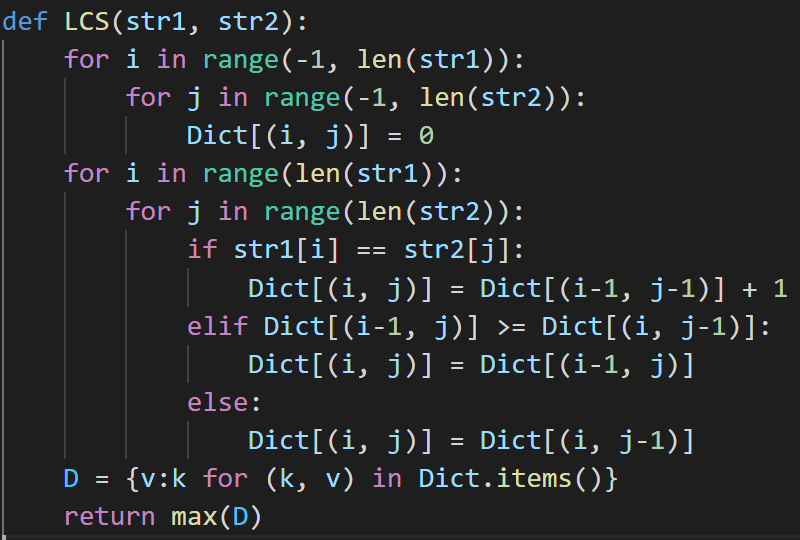
\includegraphics[height=10\baselineskip]{Intro to Algorithm/LCS.png}
\end{minipage}
\par
Caution: In the process of separating the problems, if we can guarantee that in the two sub-problems generated, one is definitely an empty problem to reach the optimal solution, we can directly turn to \textbf{Greedy Algorithm}. 
\section{Catalan Number}
We are interested in the number of different binary trees with $n$ nodes, which following will deduce. The binary tree mentioned above can be expressed as the combination of a root node and the summation of two sub-trees.
\begin{equation}
\begin{aligned}
    b_n = \sum_{i=0}^{n-1}b_ib_{n-i-1} \\
    \text{Base Case:}~~b_0 = 1
\end{aligned}
\end{equation}
The generating function of the sequence will give
\begin{equation}
    G(b, x) = \sum_{n=0}^{\infty} b_nx^n
\end{equation}
An implicit feature of $G(b,x)$ is
\begin{equation}
\begin{aligned}
    G(b,x) &= \sum_{n=1}^{\infty}\bigg(\sum_{i=0}^{n-1}b_ib_{n-i-1}\bigg)x^n + b_0\\
    &=  \sum_{n=0}^{\infty} \bigg( \sum_{i=0}^n b_ib_{n-i} \bigg) x^{n+1} + 1 \\
    &= x \cdot \sum_{n=0}^{\infty} \bigg( \sum_{i=0}^n b_ib_{n-i} \bigg) x^{n} + 1 \\
    &= xG^2(b,x) + 1 \\
    \text{Or,}~~G(b,x) &= \frac{1-\sqrt{1-4x}}{2x} \\
    &= \frac{1}{2x} \bigg(1-\big(1-2x-\sum_{n=2}^{\infty} \frac{(2n-3)!}{2^{2n-2}(n-2)!}\frac{1}{n!}(4x)^n \big)\bigg)  \\
    &= \sum_{k=0}^{\infty} \frac{(2n)!}{n!n!}\frac{1}{n+1}x^n
\end{aligned}
\end{equation}
Compare (29) and (30) we obtain
\begin{equation}
\begin{aligned}
    b_n = \frac{(2n)!}{n!n!}\frac{1}{n+1} &= \frac{1}{n+1} C_{2n}^{n} \\
    &= \frac{1}{n+1}\frac{\sqrt{4\pi n}(\frac{2n}{e})^{2n}(1+\Theta(\frac{1}{n})}{(\sqrt{2\pi n}(\frac{n}{e})^n(1+\Theta(\frac{1}{n}))^2}\\
    &= \frac{4^n}{\sqrt{\pi} n^{\frac{3}{2}}}\bigg(1+O(\frac{1}{n})\bigg)
\end{aligned}
\end{equation}
Hence we obtain the exact growing order of a binary search tree of n nodes.
\section{Longest Common Sub-string with $k$ Mismatches}
\subsection{A Degraded Model}
If there is no `$k$ mismatches' condition, the state shifting equation will be
\begin{equation}
\text{LCS}[i, j] = \left\{
\begin{aligned}
    &\text{LCS}[i-1 ,j-1],~~~\text{if str1[i] $\neq$ str2[j]} \\
    &\text{max}\{\text{LCS}[i-1, j-1] + 1,~ \text{LCS}[i-1,j],~\text{LCS}[i,j-1]\},~~~\text{if str1[i] == str2}\\
\end{aligned}
\right.
\end{equation}
With the base case
\begin{equation}
    \text{LCS}[0, j] == \text{LCS}[i,0] == 0 \notag
\end{equation}
\subsection{$k$ Mismatches}
Compared to the degraded model, some limitations are added such that
\begin{gather}
    \bigg|\bigg|\bigg\{0\leq h\leq l-1\bigg|str1[i-h] \neq str2[j-h]\bigg\}\bigg|\bigg|\leq k,~~~0\leq i<n,~~0\leq j <m \\
    \text{LCS}[i,j] = \text{max}\{l~|~l\leq \text{min}(i,j)+1\}
\end{gather}
\end{document}